\documentclass[preprint,12pt]{elsarticle}
\usepackage[a4paper,left=2.5cm,right=2.5cm,top=2.5cm,bottom=3cm,footskip=1.6cm]{geometry}
\usepackage{array}
\usepackage{xr-hyper}
\usepackage[hidelinks]{hyperref}
\externaldocument{../main}
\biboptions{numbers,sort&compress}
\emergencystretch=3em
\renewcommand{\topfraction}{0.85}
\usepackage{amsmath,amssymb,amsthm,booktabs,graphicx,xcolor,adjustbox}
\usepackage{tikz}
\usetikzlibrary{arrows.meta,decorations.pathreplacing,calc,fit,backgrounds,shadows}
\newtheorem{theorem}{Theorem}
\newtheorem{proposition}{Proposition}
\newtheorem{lemma}{Lemma}
\newtheorem{corollary}{Corollary}
\newtheorem{definition}{Definition}
\newtheorem{remark}{Remark}
\theoremstyle{definition}
\newcommand{\todo}[1]{\textcolor{red}{[TODO: #1]}}
\newcommand{\E}{\mathbb{E}}
\newcommand{\Binfo}{\mathcal{B}_{\mathrm{info}}}
\newcommand{\Istate}{\mathcal{I}_{\mathrm{state}}}
\newcommand{\Ikin}{\mathcal{I}_{\mathrm{kin}}}
\newcommand{\etaPIE}{\eta_{\mathrm{info}}}
\DeclareMathOperator{\Mon}{Mon}
\DeclareMathOperator{\Var}{Var}

\begin{document}
\begin{center}\textbf{Supplementary material to ``Information Budgets of Trajectory Health Indicators for Remaining Useful Life Prediction''}\end{center}
\medskip
\section*{S1. Initial benchmark protocol (P1)}
Abbreviations are those of the main text: health indicator (HI), remaining useful life (RUL), root mean squared error (RMSE), mean absolute error (MAE), continuous ranked probability score (CRPS), physics-guided information bottleneck (PGIB), variational information bottleneck (VIB), $\beta$-variational autoencoder ($\beta$-VAE), first-principal-component HI (PCA-HI), gated recurrent unit (GRU), Center for Advanced Life Cycle Engineering (CALCE), and the FEMTO-ST/PRONOSTIA bearings (FEMTO); the age-only baseline is the lifetime distribution conditioned on survival to the current age.

The first benchmark used a simpler protocol (P1). Every HI was calibrated on in-sample training paths, the plain first-hitting-time distribution (\ref{eq:mixig}) was used without age fusion, and the predictive grid extended to three times the held-out unit's own life, which leaks the length of the test unit into the support of the predictive distribution (removed in P2). The pilot on NASA B0005, the results below and the observation that the age-only baseline is competitive motivated P2. The P1 results are reported for completeness and are not used for the conclusions of the main text.

\paragraph{Pilot run} A pilot on the NASA B0005 fold, with a GRU-only encoder and $\beta\in\{0.003,0.03,0.3\}$, gave a PGIB RMSE of $56.3$ cycles and zero interval coverage, with the selected $\beta$ at the edge of the grid. The selection grid was therefore extended and the feed-forward encoder added as a candidate. Both changes are chosen per fold by inner validation, but the decision to introduce them was made after seeing a held-out result for one fold. No baseline was modified, and no change was made after the full runs reported below; the bearing experiments were run once with the final protocol.

\begin{table}
\caption{Protocol P1, battery benchmarks, leave-one-unit-out (mean $\pm$ standard deviation over seeds). RMSE, MAE and CRPS in cycles.}
\centering\small
\adjustbox{max width=\linewidth}{\begin{tabular}{l c c c c c c c c}
\hline
\multicolumn{9}{l}{NASA PCoE (leave-one-unit-out)}\\
 Method & Mon & Tre & Pro & RMSE & MAE & PICP [\%] & PINAW & CRPS \\
\hline
Age-only reference (no sensors) & -- & -- & -- & 39.8 & 34.7 & -- & -- & -- \\
PCA-HI & 0.27 & 0.85 & 0.77 & 17.8 & 14.0 & 97 & 2.52 & 11.1 \\
Geo-opt HI & 0.21 & 0.93 & 0.95 & 21.9 & 17.0 & 90 & 2.43 & 12.8 \\
$\beta$-VAE-HI & 0.30$\pm$0.01 & 0.71$\pm$0.00 & 0.95$\pm$0.01 & 30.8$\pm$0.8 & 26.0$\pm$0.5 & 95$\pm$1 & 2.06$\pm$0.08 & 17.6$\pm$0.5 \\
VIB-HI (no physics prior) & 1.00 & 1.00$\pm$0.00 & 0.67$\pm$0.03 & 33.3$\pm$2.8 & 27.7$\pm$2.1 & 88$\pm$4 & 3.47$\pm$0.10 & 20.5$\pm$2.3 \\
PGIB-HI & 1.00 & 1.00$\pm$0.00 & 0.67$\pm$0.01 & 47.6$\pm$2.1 & 42.3$\pm$1.9 & 42$\pm$3 & 2.39$\pm$0.15 & 34.3$\pm$1.5 \\
\hline
\end{tabular}
}\\[4pt]
\adjustbox{max width=\linewidth}{\begin{tabular}{l c c c c c c c c}
\hline
\multicolumn{9}{l}{CALCE CS2 (4 cells, 1C/1C) (leave-one-unit-out)}\\
 Method & Mon & Tre & Pro & RMSE & MAE & PICP [\%] & PINAW & CRPS \\
\hline
Age-only reference (no sensors) & -- & -- & -- & 49.3 & 43.8 & -- & -- & -- \\
PCA-HI & 0.05 & 0.72 & 0.83 & 130.5 & 110.4 & 92 & 2.74 & 82.3 \\
Geo-opt HI & 0.39 & 0.95 & 0.98 & 117.2 & 86.8 & 90 & 3.20 & 69.2 \\
$\beta$-VAE-HI & 0.02$\pm$0.01 & 0.72$\pm$0.01 & 0.80$\pm$0.01 & 163.7$\pm$0.7 & 148.0$\pm$0.9 & 83$\pm$1 & 1.87$\pm$0.02 & 111.1$\pm$0.7 \\
VIB-HI (no physics prior) & 1.00 & 1.00$\pm$0.00 & 0.92$\pm$0.01 & 53.2$\pm$0.9 & 47.2$\pm$1.4 & 71$\pm$4 & 1.24$\pm$0.13 & 38.4$\pm$0.7 \\
PGIB-HI & 1.00 & 1.00$\pm$0.00 & 0.95$\pm$0.01 & 33.0$\pm$4.9 & 29.9$\pm$3.9 & 55$\pm$8 & 0.34$\pm$0.02 & 22.6$\pm$3.1 \\
\hline
\end{tabular}
}\\[4pt]
\adjustbox{max width=\linewidth}{\begin{tabular}{l c c c c c c c c}
\hline
\multicolumn{9}{l}{CALCE CS2 (6 cells, incl. 0.5C-discharge CS2\_33/34) (leave-one-unit-out)}\\
 Method & Mon & Tre & Pro & RMSE & MAE & PICP [\%] & PINAW & CRPS \\
\hline
Age-only reference (no sensors) & -- & -- & -- & 54.7 & 50.0 & -- & -- & -- \\
PCA-HI & 0.13 & 0.28 & 0.21 & 191.8 & 172.0 & 50 & 0.99 & 149.6 \\
Geo-opt HI & 0.39 & 0.95 & 0.98 & 106.9 & 82.7 & 95 & 3.11 & 63.7 \\
$\beta$-VAE-HI & 0.05$\pm$0.02 & 0.52$\pm$0.10 & 0.33$\pm$0.04 & 201.6$\pm$5.3 & 179.9$\pm$5.0 & 48$\pm$0 & 1.46$\pm$0.18 & 156.1$\pm$3.1 \\
VIB-HI (no physics prior) & 1.00 & 1.00$\pm$0.00 & 0.87$\pm$0.02 & 69.7$\pm$6.0 & 54.4$\pm$8.8 & 90$\pm$5 & 2.24$\pm$0.23 & 44.9$\pm$4.8 \\
PGIB-HI & 1.00 & 1.00$\pm$0.00 & 0.91$\pm$0.01 & 50.4$\pm$4.4 & 44.7$\pm$5.1 & 69$\pm$5 & 0.58$\pm$0.02 & 33.4$\pm$4.2 \\
\hline
\end{tabular}
}
\label{tab:benchv1}
\end{table}

\begin{table}
\caption{Protocol P1, FEMTO bearing benchmarks. RMSE, MAE and CRPS in $10$~s snapshots.}
\centering\small
\adjustbox{max width=\linewidth}{\begin{tabular}{l c c c c c c c c}
\hline
\multicolumn{9}{l}{FEMTO bearings, condition 1 (7 units) (leave-one-unit-out)}\\
 Method & Mon & Tre & Pro & RMSE & MAE & PICP [\%] & PINAW & CRPS \\
\hline
Age-only reference (no sensors) & -- & -- & -- & 602.5 & 515.4 & -- & -- & -- \\
PCA-HI & 0.06 & 0.56 & 0.70 & 784.5 & 663.2 & 93 & 2.80 & 485.7 \\
Geo-opt HI & 0.04 & 0.29 & 0.39 & 770.2 & 623.3 & 91 & 3.34 & 459.1 \\
$\beta$-VAE-HI & 0.07$\pm$0.02 & 0.58$\pm$0.01 & 0.73$\pm$0.01 & 779.8$\pm$51.1 & 664.4$\pm$35.6 & 91$\pm$3 & 2.69$\pm$0.13 & 492.4$\pm$20.6 \\
VIB-HI (no physics prior) & 1.00 & 1.00$\pm$0.00 & 0.71$\pm$0.02 & 570.1$\pm$56.0 & 471.0$\pm$50.7 & 78$\pm$5 & 3.04$\pm$0.21 & 365.6$\pm$44.1 \\
PGIB-HI & 1.00 & 1.00$\pm$0.00 & 0.71$\pm$0.02 & 524.5$\pm$45.3 & 423.6$\pm$37.3 & 75$\pm$5 & 2.65$\pm$0.10 & 336.5$\pm$31.8 \\
\hline
\end{tabular}
}\\[4pt]
\adjustbox{max width=\linewidth}{\begin{tabular}{l c c c c c c c c}
\hline
\multicolumn{9}{l}{FEMTO bearings, condition 2 (7 units) (leave-one-unit-out)}\\
 Method & Mon & Tre & Pro & RMSE & MAE & PICP [\%] & PINAW & CRPS \\
\hline
Age-only reference (no sensors) & -- & -- & -- & 664.4 & 584.6 & -- & -- & -- \\
PCA-HI & 0.04 & 0.43 & 0.17 & 613.9 & 487.6 & 54 & 2.25 & 433.9 \\
Geo-opt HI & 0.06 & 0.37 & 0.46 & 559.2 & 457.1 & 73 & 2.33 & 356.5 \\
$\beta$-VAE-HI & 0.06$\pm$0.01 & 0.46$\pm$0.05 & 0.42$\pm$0.16 & 539.8$\pm$31.7 & 439.6$\pm$24.6 & 70$\pm$2 & 2.01$\pm$0.06 & 348.6$\pm$26.1 \\
VIB-HI (no physics prior) & 1.00 & 0.99$\pm$0.00 & 0.39$\pm$0.02 & 616.8$\pm$1.5 & 493.8$\pm$1.5 & 41$\pm$1 & 2.62$\pm$0.23 & 451.1$\pm$3.2 \\
PGIB-HI & 1.00 & 0.99$\pm$0.00 & 0.46$\pm$0.02 & 621.8$\pm$4.3 & 498.2$\pm$8.1 & 36$\pm$2 & 2.25$\pm$0.01 & 464.3$\pm$7.9 \\
\hline
\end{tabular}
}
\label{tab:benchbv1}
\end{table}

\begin{table}
\caption{Protocol P1, lower bound on the information implied by the achieved error (Theorem~\ref{thm:bound}(b)), in nats; $<0$: uninformative. $h(T)$: entropy of the pooled held-out RUL.}
\centering\small
\begin{tabular}{l c c c c c c}
\hline
Dataset & $h(T)$ & PCA & Geo-opt. & $\beta$-VAE & VIB & PGIB \\
\hline
NASA & 4.36 & 0.06 & $<0$ & $<0$ & $<0$ & $<0$ \\
CALCE (4) & 5.67 & $<0$ & $<0$ & $<0$ & 0.27 & 0.76 \\
CALCE (6) & 5.66 & $<0$ & $<0$ & $<0$ & $<0$ & 0.32 \\
FEMTO c.\,1 & 7.24 & $<0$ & $<0$ & $<0$ & $<0$ & $<0$ \\
FEMTO c.\,2 & 7.04 & $<0$ & $<0$ & $<0$ & $<0$ & $<0$ \\
\hline
\end{tabular}

\label{tab:certv1}
\end{table}

\begin{figure}[!tb]
\centering
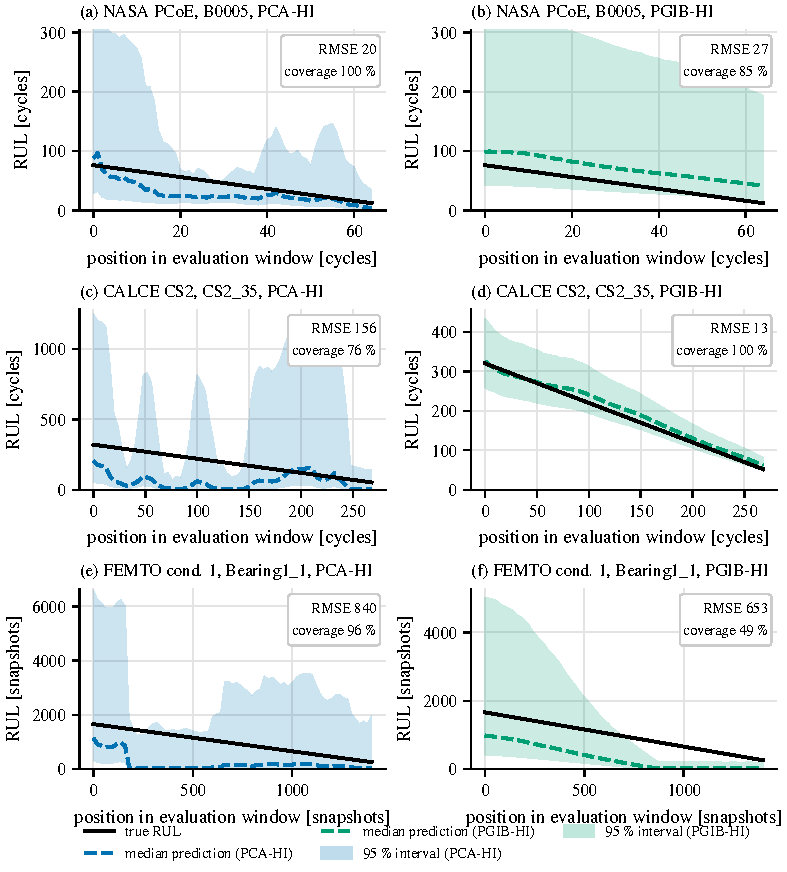
\includegraphics[width=\textwidth]{../figs/fig_bench}
\caption{Example RUL predictions with $95\%$ intervals on one held-out unit per data set (NASA B0005, CALCE CS2\_35, FEMTO Bearing1\_1), for PCA-HI (left) and PGIB (right); each panel gives the RMSE and the coverage on that unit.}
\label{fig:benchv1}
\end{figure}

\paragraph{Results under P1} The outcome depends on the data set (Tables~\ref{tab:benchv1} and \ref{tab:benchbv1}, Figure~\ref{fig:benchv1}), and the age-only baseline is needed to read it. On NASA the RMSE of the age-only baseline is $39.8$ cycles; PCA-HI ($17.8$), the Geo-opt HI ($21.9$), the $\beta$-VAE ($30.8$) and VIB ($33.3$) outperform it, whereas the PGIB ($47.6$) does not, and its intervals cover only $42\%$ of the true RULs. On CALCE the RMSE of the age-only baseline is $49.3$; only the PGIB ($33.0$) outperforms it clearly, while PCA-HI, the Geo-opt HI and the $\beta$-VAE ($117$ to $164$) are considerably worse than the age-only baseline. With the two $0.5$C-discharge cells added, the PGIB keeps the lowest RMSE ($50.4$) but its margin over the age-only baseline ($54.7$) is only $8\%$. On bearings the RMSE of the age-only baseline ($602$ and $664$ snapshots for conditions 1 and 2) is comparable to the standard deviation of the pooled RUL, and most HIs do no better: the PGIB has the lowest RMSE in condition 1 ($524.5$, $13\%$ below the age-only baseline) but gives almost no benefit in condition 2 ($621.8$ against $664$). Two long-lived units dominate the pooled error in condition 2.

The ablations (in the supplied result files) support the bottleneck on all five sets (for example RMSE $54.4\to47.6$ on NASA and $42.3\to33.0$ on CALCE) and the epistemic drift variance for coverage (for example $14\to42\%$ on NASA). The physics prior helps on CALCE and FEMTO condition 1 but not on NASA or FEMTO condition 2. With only three to six training units per fold, the validation signal that selects the encoder is itself noisy; on NASA it chose the strongest compression ($\beta=30$), at the edge of the grid, in all eight selections.

\paragraph{Geometric scores versus error} Across the five HIs of each data set, the rank correlation between the geometric score $\Mon+\mathrm{Tre}+\mathrm{Pro}$ and the RMSE is $+0.90$ on NASA (a higher geometric score goes with a larger error), $-1.00$ on CALCE, $-0.90$ on six-cell CALCE, $-0.60$ on FEMTO condition 1 and $+0.60$ on condition 2. The geometric criteria therefore did not rank the HIs consistently by prognostic error. This is an association over five methods per data set and not evidence for the mechanism of Theorem~\ref{thm:paradox}: the VIB and PGIB HIs have $\Mon\approx\mathrm{Tre}\approx1$ because their velocity is constrained to be positive, not because of a squeeze.

\end{document}
